% !TEX spellckeck=en_GB

\section{Clustering using a pre-trained model}\label{sec:vgg_cluster}

As in chapter \ref{ch:architectures}, we also use the VGG16 pre-trained network as a baseline for the clustering performance. We begin by considering a classical K-means approach to clustering. However, the output from the VGG16 network is very high dimensional with output vectors in $\R^{8192}$. One of the primary concerns is then the curse of dimensionality, where the ratio of distances goes to one with increasing dimensionality as shown by \citet{Aggarwal}. However, one of the central caveats to the authors  finding is that the elements are uniformly distributed in the latent space. It is then possible that all the class information lies in some sub-space of the latent data. To investigate this, we perform clustering analysis using the full representation and the $10^2$ first principal components only. 

\subsection{K-means}

We begin by investigating the K-means clustering algorithm on the VGG16 latent space. As in chapter \ref{chap:classification} the VGG16 model is pre-trained on the imagenet dataset creating a set of vectors $\boldsymbol{x} \in \R^{8192}$. To cluster we use \lstinline{scikit-learn} implementation of the K-means algorithm, with default parameters \cite{Pedregosa2011}. The results of the clustering runs are included in table \ref{tab:clstr_vgg}. We observe that we are able to attain near-perfect clustering on simulated data and that there is a sharp decline in performance as we add noise by moving to the filtered and full datasets. 

\begin{table}[H]
\centering 
\caption[K-means on pre-trained model]{K-means clustering results on AT-TPC event data. We observe that the performance predictably decreases with the amount of noise in the data.}\label{tab:clstr_vgg}
\begin{tabular}{lll}
\toprule
{} & Accuracy &   ARI \\
\midrule
Simulated &     0.97 &  0.89 \\
Filtered  &     0.74 &  0.39 \\
Raw       &     0.59 &  0.17 \\
\bottomrule
\end{tabular}

\end{table}

In addition to the performance measures reported in table \ref{tab:clstr_vgg}, it is interesting to observe which samples are being wrongly assigned. We achieve this by tabulating the assignments of samples relative to their ground truth labels. From these tables, we can infer which classes are more or less entangled with others. We tabulate the results for each dataset is in figure \ref{fig:clster_confmat}. We observe that the proton class is consistently assigned in a pure cluster. Purity is inferred by how much spread there is in the column between the ground truth labels. A high-quality cluster will, in addition to being pure, also capture most entries the class represented by the cluster. For example, consider the row corresponding to the proton class in figure \ref{fig:clster_confmat}. The column corresponding to the largest entry in the proton row has zero other predicted classes in it. From this, we conclude that the proton cluster is a high quality, high purity cluster. 

\begin{figure}
\centering

	\subfloat{
	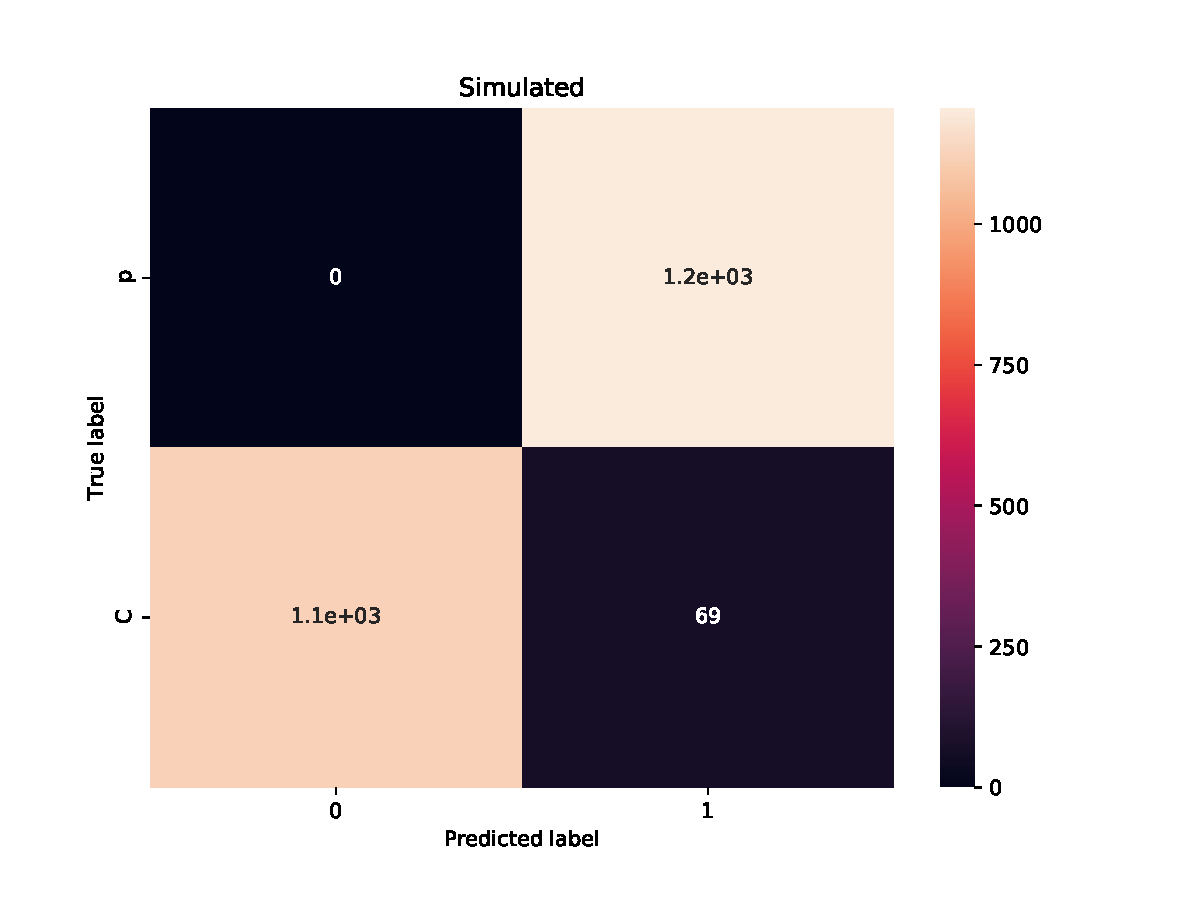
\includegraphics[width=0.35\textwidth]{./plots/Simulatedvgg_pca_conf_mat.pdf}

}
	\hspace{-1cm}
	\subfloat{
	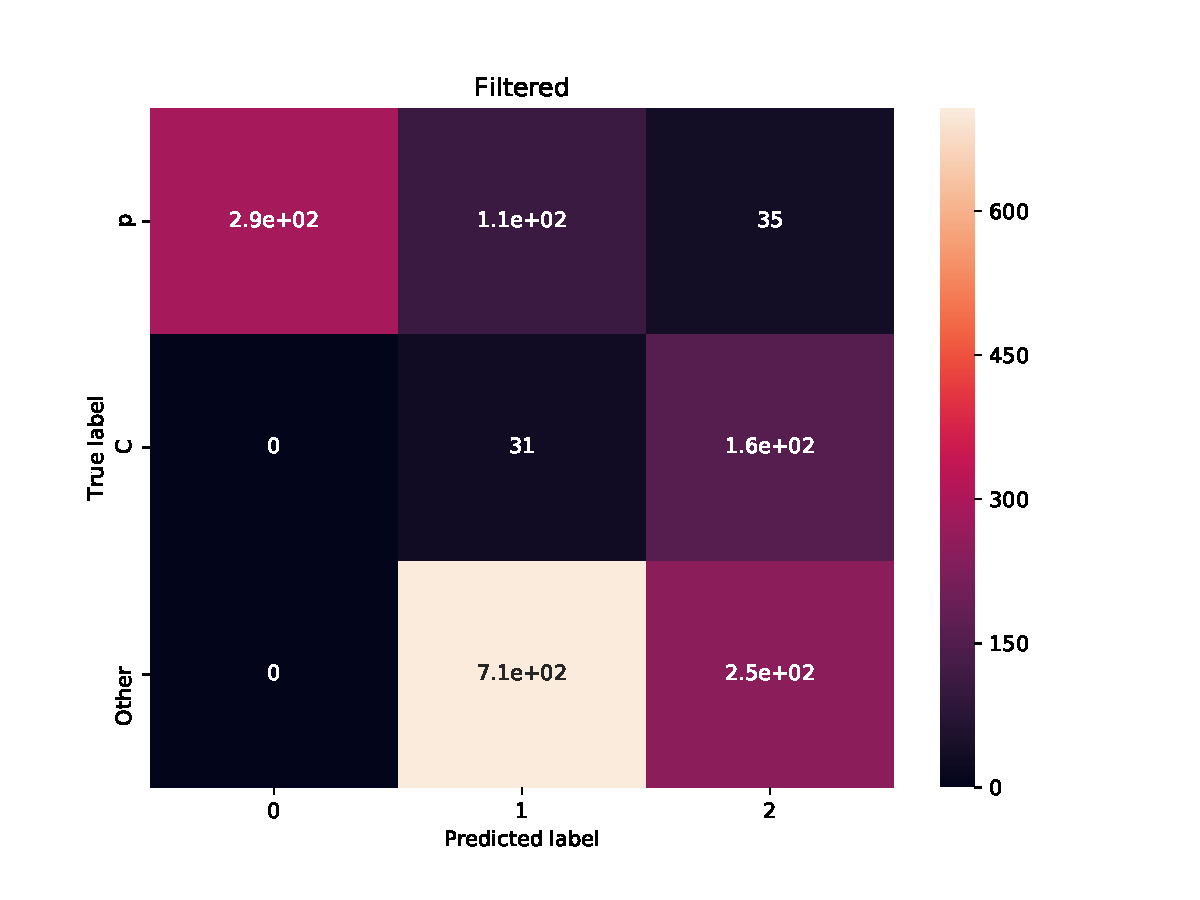
\includegraphics[width=0.35\textwidth]{plots/Filteredvgg_pca_conf_mat.pdf}
}
	\hspace{-1cm}
	\subfloat{
	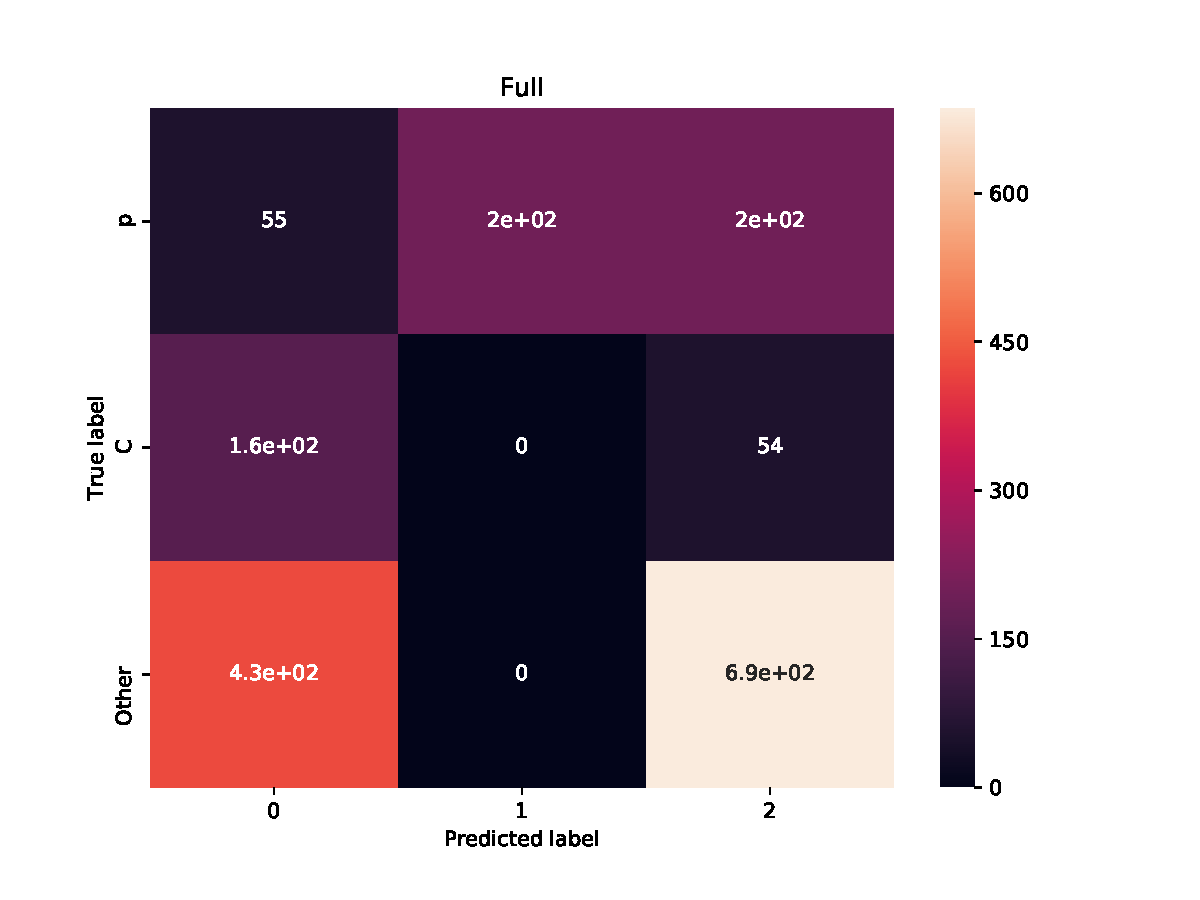
\includegraphics[width=0.35\textwidth]{plots/Fullvgg_pca_conf_mat.pdf}
}
\caption[Pre-trained network - confusion matrices]{Confusion matrices for the K-means clustering of simulated, filtered and full AT-TPC events. The true labels indicate samples belonging to the p (proton), carbon (C), or other classes. }\label{fig:clster_confmat}
\end{figure}

We repeat this analysis using a PCA dimensionality reduction on the latent space of the VGG16 model. This is done to estimate to what degree the class separating information is encoded in the entirety of the latent space, or in some select regions. The results from the PCA analysis were virtually identical to the results sans the PCA, and so we omit them for brevity. 

Furthermore, we wish to characterize further the clusters presented in figure \ref{fig:clster_confmat}. To achieve this, we sample from the proton samples belonging to different clusters for the filtered and full data.

\begin{figure}
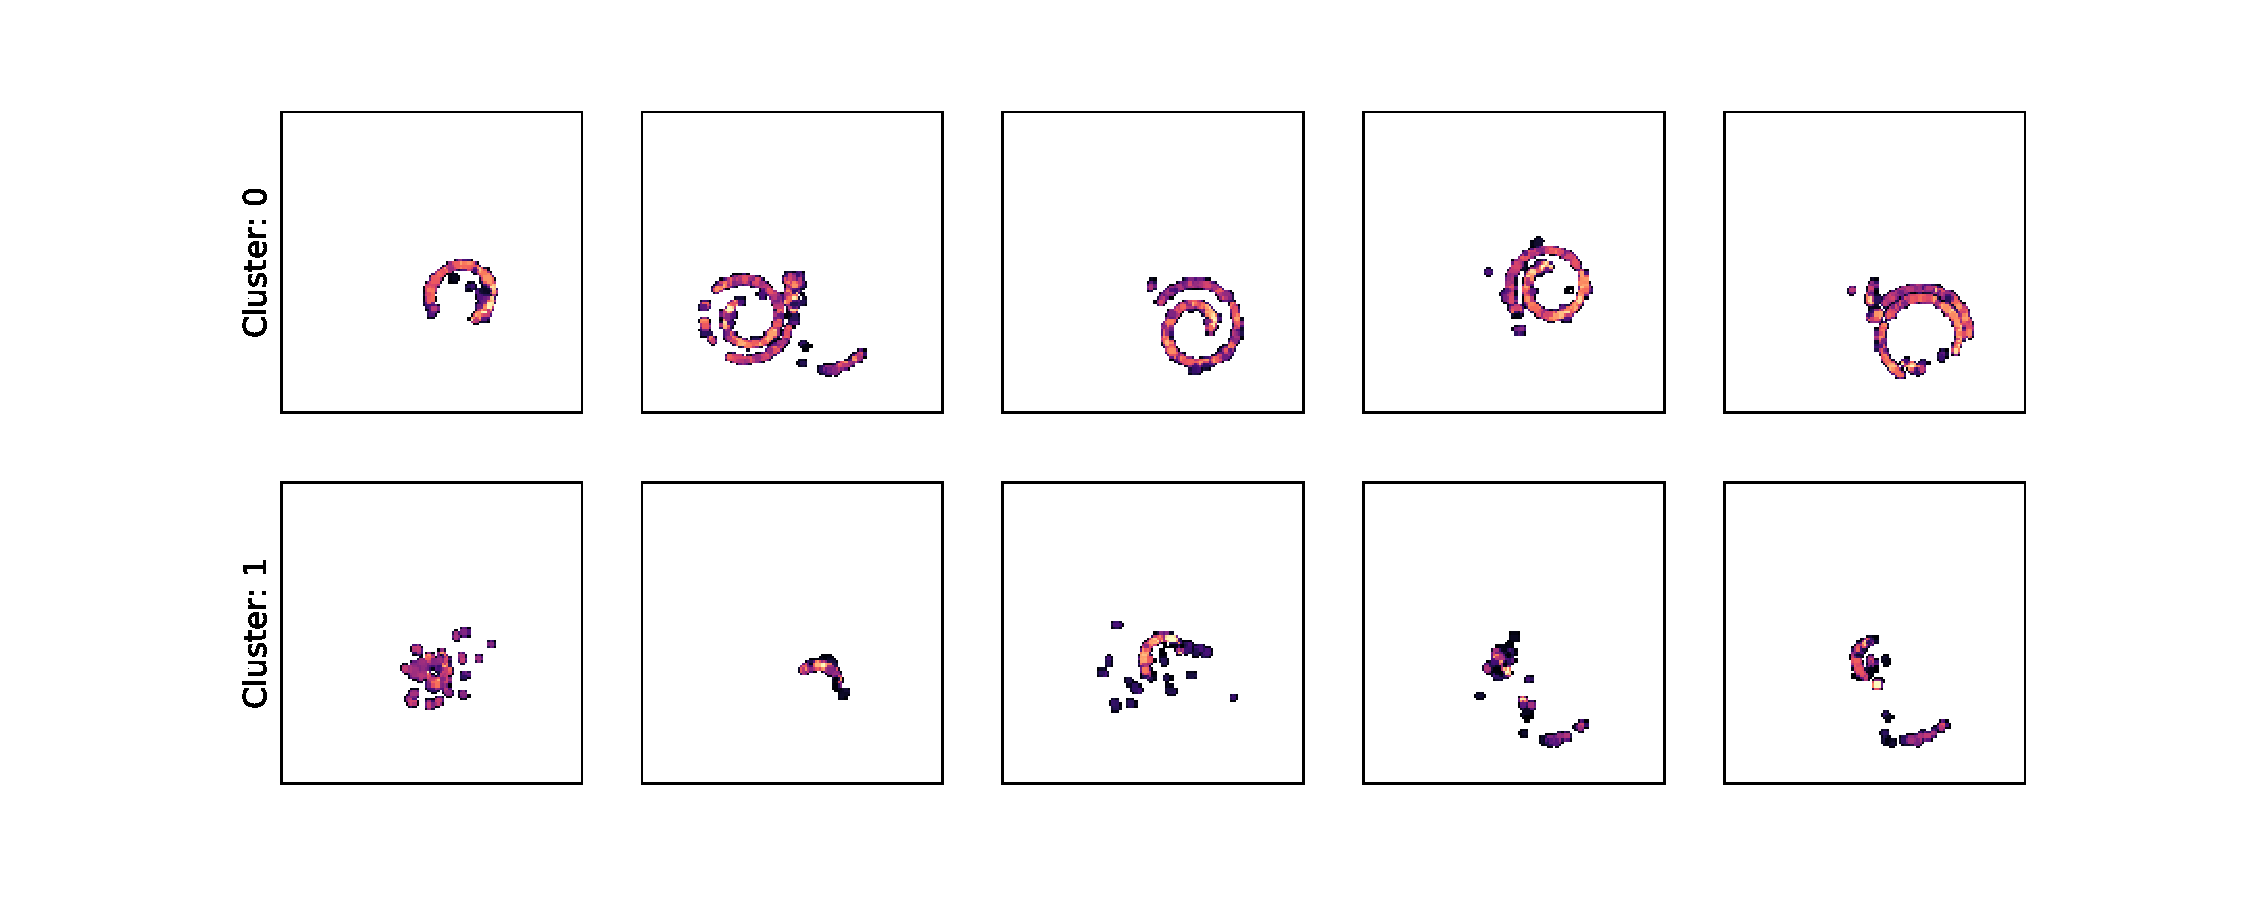
\includegraphics[width=\textwidth]{plots/filtered_vgg_cluster_repr.pdf}
\caption[Filtered proton samples by cluster belonging]{Illustrating a sample of proton events from different K-means clusters from the filtered dataset. Each row belongs to a single cluster corresponding to the filtered confusion matrix in figure \ref{fig:clster_confmat}}\label{fig:filtered_vgg_clster_repr}
\end{figure} 

\begin{figure}
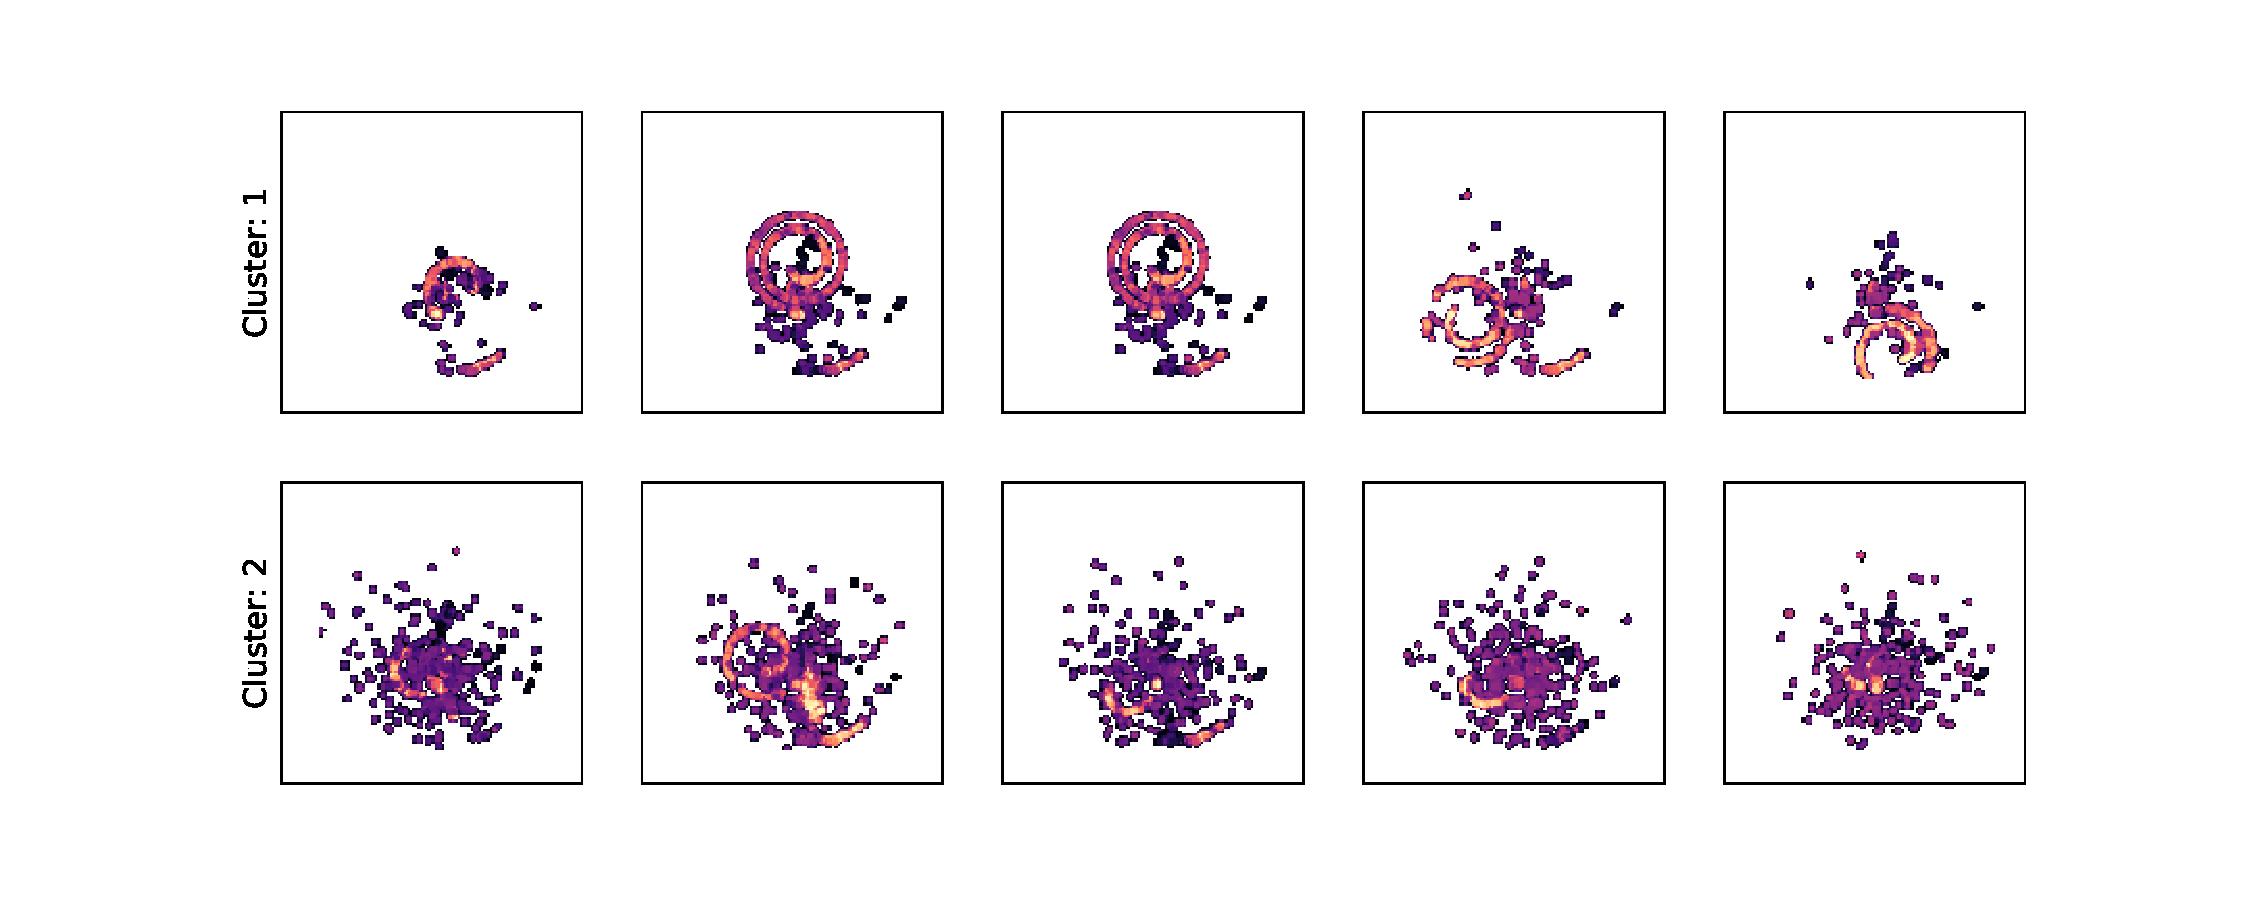
\includegraphics[width=\textwidth]{plots/full_vgg_cluster_repr.pdf}
\caption[Full proton samples by cluster belonging]{Illustrating a sample of proton events from different K-means clusters from the full dataset. Each row belongs to a single cluster corresponding to the full confusion matrix in figure \ref{fig:clster_confmat}}\label{fig:full_vgg_clster_repr}
\end{figure} 

In addition to the results presented in this section, we performed clustering with a number of different algorithms included in the \lstinline{scikit-learn} package. None of them provided any notable differences from the K-means results or were significantly worse. Notably, the DBSCAN algorithm failed to provide any useful clustering results. We find this important as one of the significant drawbacks of K-means, and the deep clustering algorithms presented in section \ref{sec:deep_clustering}, is that they are all dependent on pre-determining the number of clusters. This is not the case for DBSCAN. 